\def\year{2015}
%File: formatting-instruction.tex
\documentclass[letterpaper]{article}
\usepackage{aaai}
\usepackage{times}
\usepackage{helvet}
\usepackage{courier}
\usepackage{graphicx}
\usepackage{subcaption}
\usepackage{}
\frenchspacing
\setlength{\pdfpagewidth}{8.5in}
\setlength{\pdfpageheight}{11in}
\pdfinfo{
/Title (Insert Your Title Here)
/Author (Put All Your Authors Here, Separated by Commas)}
\setcounter{secnumdepth}{1}  
 \begin{document}
% The file aaai.sty is the style file for AAAI Press 
% proceedings, working notes, and technical reports.
%
\title{Combining Learning and Evolution in OpenNERO}
\author{Jacob Robertson \and Yun Wu\\
Department of Computer Science\\
University of Texas at Austin\\
}
\maketitle
\begin{abstract}
\begin{quote}
Evolution of agents that learn during their ``lifetimes'' is a model interesting in both its interactions between evolution and learning as well as in its qualities as an analog for biological evolution. NEAT+Q is an existing algorithm combining neuro-evolution and reinforcement learning. The OpenNERO platform is a robust simulation in a large continuous-valued setting making it interesting and useful for research in neural networks and artificial intelligence. We adapt NEAT+Q to continuous action spaces and implement the resulting algorithm in OpenNERO. In doing so we show the usefulness of combining evolution and learning, especially in complex tasks with local optima.
\end{quote}
\end{abstract}

\section{Introduction}
Evolutionary algorithms have presented themselves as an interesting and useful method for the training of neural networks. Typically speaking the evolved genomes in some way represent the final behavior of agents being evaluated for fitness. Should we choose to take the evolutionary analog a step further, we may consider agents that learn during their ``lifetime'' as part of an evolutionary process.  In computational models, non-biological models such as Lamarckian evolution, in which the expressed behavior of an agent is written back to its genome before reproduction.

There are multiple methods for combining learning and evolution in this manner, including supervised learning using labels for some task assumed to be positively related to evolutionary goals \cite{nolfi1994learning}, or using samples from human interaction to learn visibly intelligent behavior \cite{bryant2007acquiring}. Evolution can be combined with reinforcement learning by evolving networks for use as Q-value approximators \cite{whiteson2006evolutionary}. Additionally, social learning schemes may be applied in multi-agent scenarios \cite{tansey2012accelerating}

OpenNERO\footnote{https://code.google.com/p/opennero/} is an open source software platform designed for research and education in Artificial Intelligence. The project is based on the Neuro-Evolving Robotic Operatives (NERO) game developed by graduate and undergraduate students at the Neural Networks Research Group and Department of Computer Science at the University of Texas at Austin. In the NERO game, The learning agents in NERO are simulated robots, and the goal is to train a team of these agents for combat. The agents are trained by a human player who is able to set positive or negative reward values for certain behaviors, such as approaching a flag, staying together as a group, firing upon enemy agents, and avoiding fire from enemy agents. This setting is continuous in its state space (an array of continuous-valued sensors), its action space (an array of actuators, in this case speed and rotation), and time. It can be used for multi-agent algorithms, including both cooperation within a team and competition between teams. Furthermore, it supports teams of agents trained through evolution through rtNEAT, an extension of the NeuroEvolution of Augmenting Topologies algorithm in which agents has individualized lifetimes as opposed to there being a discrete set of generations, as well as Q-learning for reinforcement learning \cite{stanley2006real}.

There appears to be some benefit to learning during evolution, though the results vary by domain and the mechanisms for benefit are not clearly understood. Furthermore, existing research into methods of combining learning and evolutions tend to examine relatively simple domains. For instance, NEAT+Q \cite{whiteson2006evolutionary} is only suitable for discrete action spaces.

This paper examines NEAT+Q, adapts it for use in continuous action spaces, and evaluates its performance in the OpenNERO environment. We show that the introduction of learning can be advantageous over simple neuro-evolution, and is particularly well-suited for more difficult tasks in which local optima may be a problem. 

\section{Background}
Let us review NEAT+Q, the basis of our implementation, as well as existing work in adapating Q-learning for continuous action spaces.

\subsection{NEAT+Q}
Temporal difference methods are well established both theoretically and empirically within reinforcement learning. In particular, Q-learning has enjoyed a significant amount of success, particularly when used with neural network function approximators. NEAT+Q takes advantage of NEAT to select the networks used for function approximation. NEAT selects network topologies and weights that are well suited to learn via backpropagation towards Q-value learning rules. The effectiveness of network Q-value approximators is senstive to the topology of the underlying network, which in this case is selected by NEAT to be useful without the need to be tuned by an experimenter. 

The NEAT+Q algorithm may be viewed from this Q-learning perspective, or from an evolutionary perspective, in which the algorithm acts as a modification of the action selection mechanism used by evolved agents. Each agent in order to select an action, activates its current sensors through its network. It then selects a random action with some probability $\epsilon$, or the action corresponding to the output with the highest activation value otherwise. It is then able to use received reward, as well as the previously seen sensors and selected action to produce a new observed Q-value for the previously taken action. This creates an error signal on the output corresponding to that action that may be backpropagated. Note that there is an implicit assumption that each output from the network corresponds to an action from a discrete set of possible actions, and that when the network represents a Q-value approximator, selecting an action with the highest activation is equivalent to selecting an action with the highest Q-value.

\subsection{Q-learning with continuous actions}
Gaskett et al. describe a system for Q-learning in continuous action spaces with neural network function approximators~\cite{gaskett1999q}. Their method makes uses of least-squares interpolator on top of the underlying network. Instead of the output layer of the network being a single output per action, the output of the network is a collection of ``wires''. Each wire represents a group of outputs: a continuous-valued action vector as well as a Q-value for that action vector. The set of wires produced by activating the network provide a set of samples for the wire-fitter to interpolate the Q-value function of the action space for a given state. Action selection may occur by choosing the action vector associated with the highest Q-value. Afterwards, the wire-fitter provides a new Q-value function based on observed rewards, and the output of the network can be backpropagated towards that new function. The new targets to be trained towards are themselves determined by gradient descent, incurring additional cost per iteration of backpropagation.

\section{Approach}
Our implementation makes use of ideas from wire-fitted Q-learning to adapt NEAT+Q to the continuous action space used by rtNEAT in OpenNERO. For brevity we will refer to our implementation as rtNEAT+Q. It is worth noting with wire-fitting that the new observation being used to update the Q-value function will always be just a new Q-value for a previously output action vector. For that action vector alone, it is simpler to just train it towards a newly observed Q-value than to use the full approach described by the wire-fitting algorithm. This is possible because it is unnecessary to compute a new target action vector to train towards. Additionally, we would like to avoid incurring the cost of a complete gradient descrent process at each action selection of our implementation.

The OpenNERO agent network's output is a continuous-valued action vector. NEAT+Q assumes a discrete action space in which each network output represents a single action. We instead use the format of the ouputs used by the wire-fitting algorithm, in which the network outputs a number of candidate action vectors and their associated Q-values. Actions are selected from these outputs in an epsilon-greedy fashion, and error is only propagated on the Q-value corresponding to the previously selected candidate. In this way we take advantage of the fact the we will always obtain a new Q-value for the previously selected action vector, but we do not apply any learning to the other candidates regardless of their similarity to the previously selected action vector. This avoids the cost of gradient descent to determine the full set of learning targets used in wire-fitting. We rely on NEAT to optimize the set of candidate actions over the course of the evolutionary process. From this approach we were able to extend the existing rtNEAT agents in OpenNERO to learn during their lifetimes and evolve in a Lamarckian fashion.

\section{Experiments and Results}
\label{sec:exp}
In this paper, we evaluate the rtNEAT+Q algorithm in OpenNERO. As shown in Figure~\ref{fig:opennero}, in our experiments we focus on the task of approaching a flag in different scenarios.
\begin{figure}[ht]
\centering
  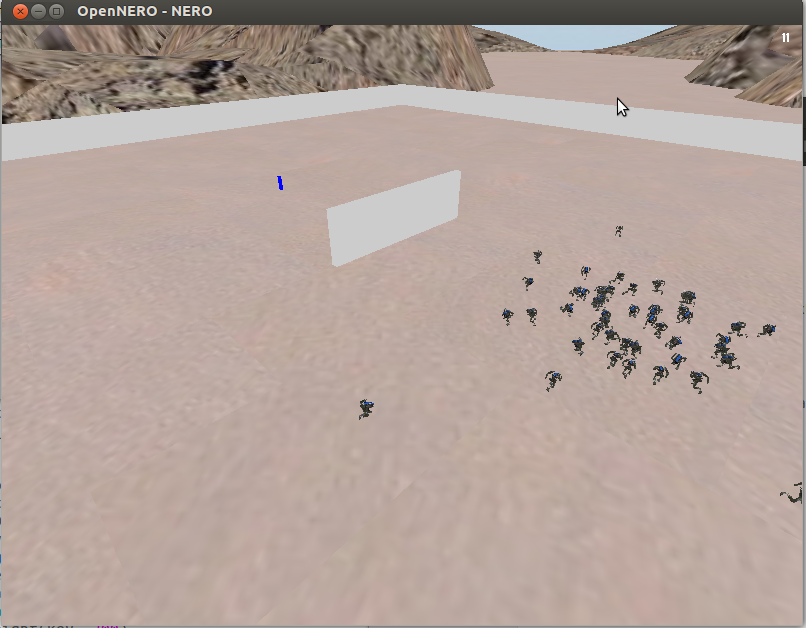
\includegraphics[width=0.7\columnwidth]{opennero.png}
\caption{OpenNERO scenario}
\label{fig:opennero}
\end{figure}

\subsection{Approaching a flag}
The first task is to run towards a flag directly. The distance between the spawn spot of agents and the flag is 141.4. Figure~\ref{fig:flag} illustrates the result. The green line is the average distance among all the agents and the blue line shows the change of the minimum distance. From Figure~\ref{fig:flag_q} we can find that the result of Q learning in continuous domain is quite unstable. rtNEAT, however, performs much better. The most fast agent gets to the flag quickly (around 25 ticks). The average distance converges at around 200 ticks when most agents has learnt to approach a flag. The combination of rtNEAT and Q learning has similar performance with rtNEAT. The average distance converges quickly but is longer than the rtNEAT agents. 
\begin{figure*}[ht]
\centering
\begin{subfigure}{0.7\columnwidth}
  \centering
  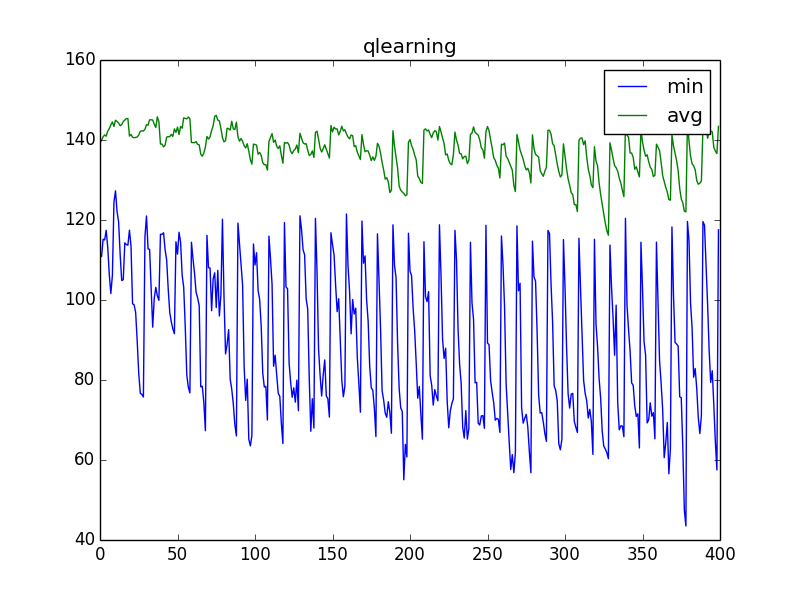
\includegraphics[width=\columnwidth]{flag_qlearning.png}
  \caption{Q Learning}
  \label{fig:flag_q}
\end{subfigure}%
\begin{subfigure}{0.7\columnwidth}
  \centering
  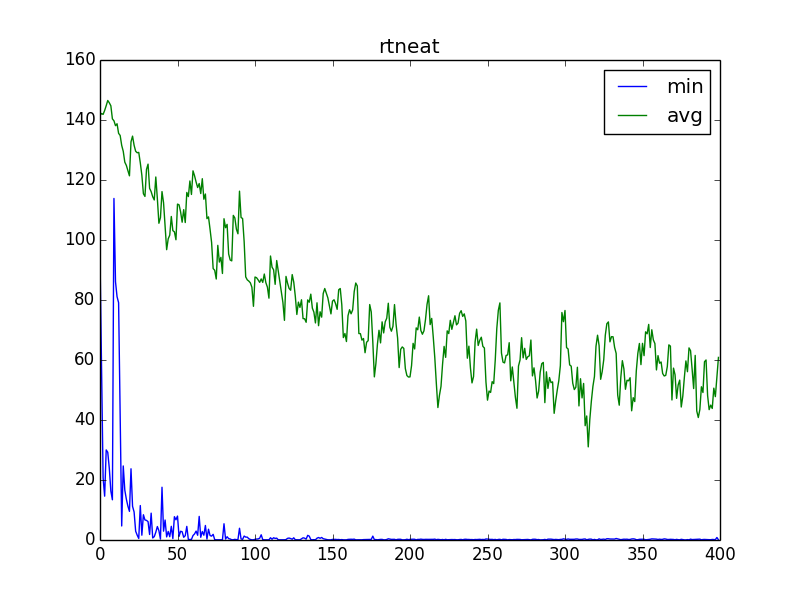
\includegraphics[width=\columnwidth]{flag_rtneat.png}
  \caption{rtNEAT}
  \label{fig:flag_neat}
\end{subfigure}
\begin{subfigure}{0.7\columnwidth}
  \centering
  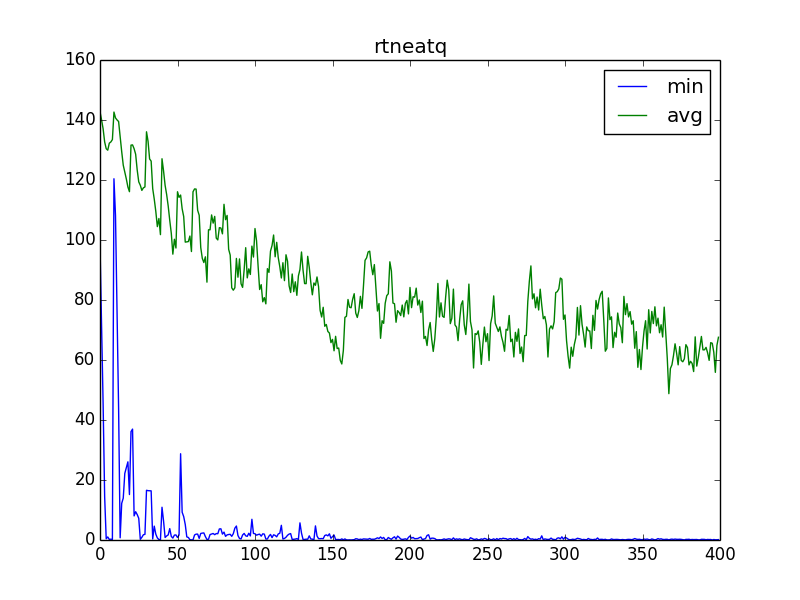
\includegraphics[width=\columnwidth]{flag_rtneatq.png}
  \caption{rtNEAT + Q Learning}
  \label{fig:flag_neatq}
\end{subfigure}
\caption{Approaching a flag}
\label{fig:flag}
\end{figure*}

\subsection{Approaching a moving flag}
We also experimented on approaching a moving flag with different algorithms(Figure~\ref{fig:moving}). Here, the location of the flag is updated randomly every 50 ticks. The minimum distance is 141 and the maximum is 283. For all three algorithm, the process of location update is the same. rtNEAT agents are able to run towards the flag within the first 50 ticks. And after every update, both minimum distance and average distance drop dramatically. The combination of rtNEAT and Q learning is able to learn the behavior within first three updates. And the average distance after 50 ticks is also longer than rtNEAT alone, which is consistent with static flag. The performance of Q learning is still unsatisfactory. The average distance does not change much after long time of training.

\begin{figure*}[ht]
\centering
\begin{subfigure}{0.7\columnwidth}
  \centering
  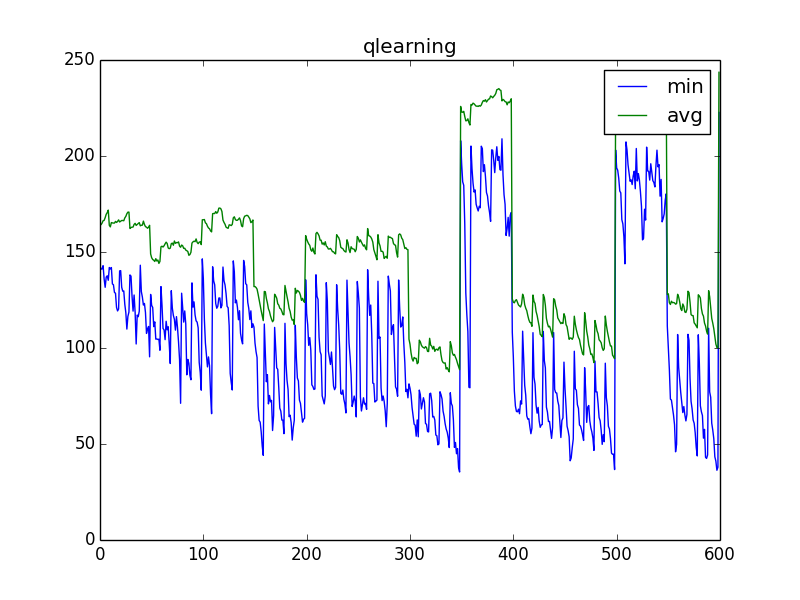
\includegraphics[width=\columnwidth]{moving_qlearning.png}
  \caption{Q Learning}
  \label{fig:moving_q}
\end{subfigure}%
\begin{subfigure}{0.7\columnwidth}
  \centering
  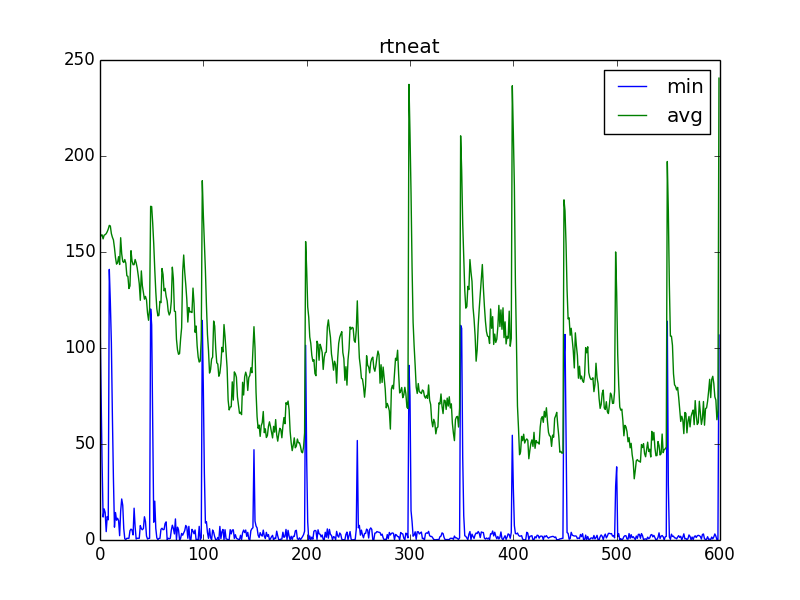
\includegraphics[width=\columnwidth]{moving_rtneat.png}
  \caption{rtNEAT}
  \label{fig:moving_neat}
\end{subfigure}
\begin{subfigure}{0.7\columnwidth}
  \centering
  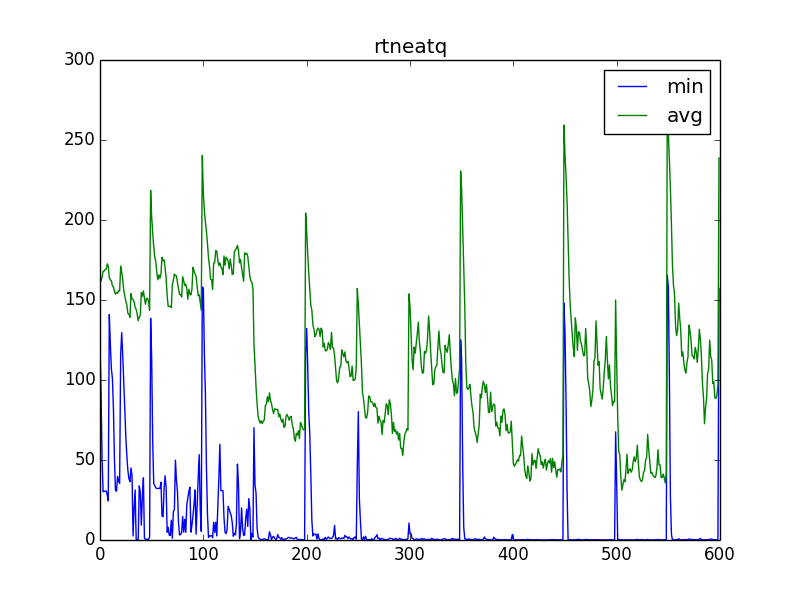
\includegraphics[width=\columnwidth]{moving_rtneatq.png}
  \caption{rtNEAT + Q Learning}
  \label{fig:moving_neatq}
\end{subfigure}
\caption{Approaching a moving flag}
\label{fig:moving}
\end{figure*}


\subsection{Approaching a flag with obstacles}
However, when it comes to more complex tasks, the benefit of learning appears. In the third experiments, the distance between agents and the flag is 267. And there is a wall with width 100 between them. Agents need to learn to get around the wall to approach the flag. As shown in Figure~\ref{fig:wall}, Q learning agents never get a chance to get close to the flag within 700 ticks. The minimum distance between agents and flag is about 170. However, from Figure~\ref{fig:wall_neat} and Figure~\ref{fig:wall_neatq}, it is clear that at first, agents learn to go directly towards flag until they are blocked by the wall. Then exploration then helps find the way around. Q learning then back propagate their network and learn the route. Finally, although rtNEAT+Q converges more slowly than rtNEAT, agents runs toward the flag more fast. The average distance of rtNEAT converges to 180 while that of rtNEAT+Q to 150. 
\begin{figure*}[ht]
\centering
\begin{subfigure}{0.7\columnwidth}
  \centering
  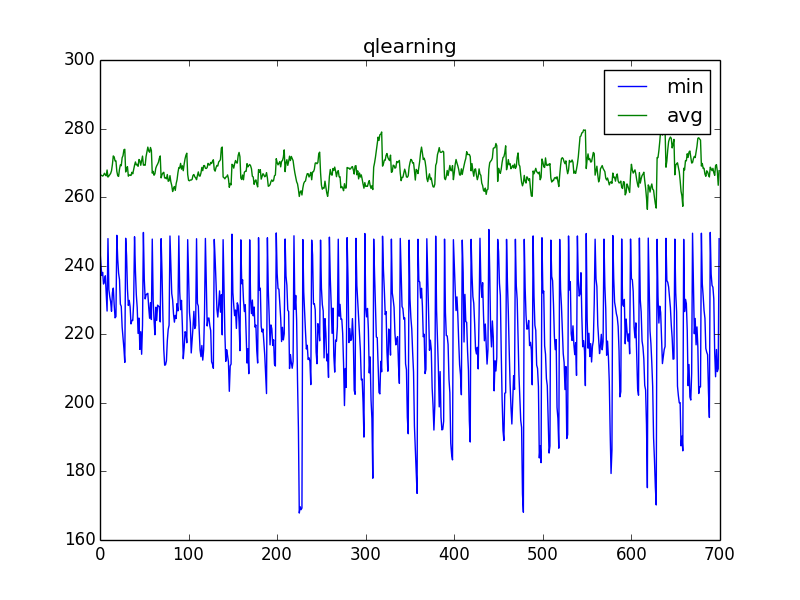
\includegraphics[width=\columnwidth]{wall_qlearning.png}
  \caption{Q Learning}
  \label{fig:wall_q}
\end{subfigure}%
\begin{subfigure}{0.7\columnwidth}
  \centering
  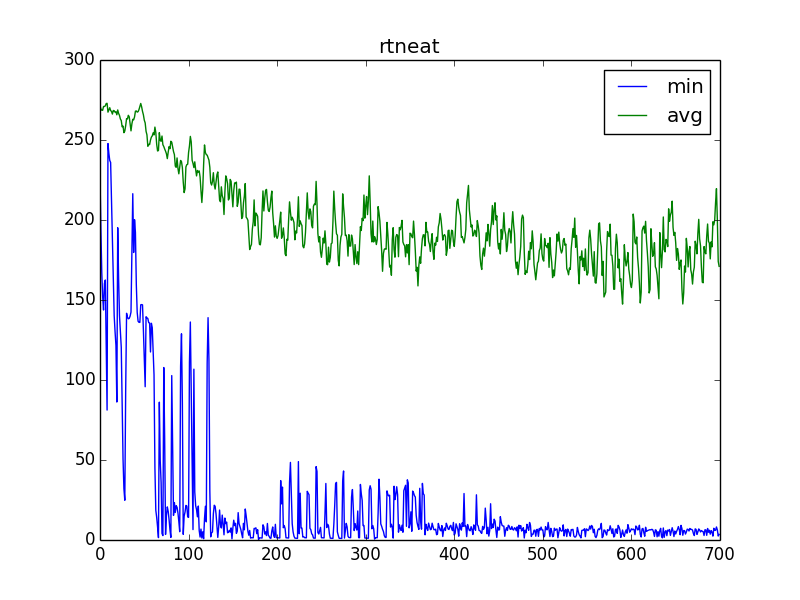
\includegraphics[width=\columnwidth]{wall_rtneat.png}
  \caption{rtNEAT}
  \label{fig:wall_neat}
\end{subfigure}
\begin{subfigure}{0.7\columnwidth}
  \centering
  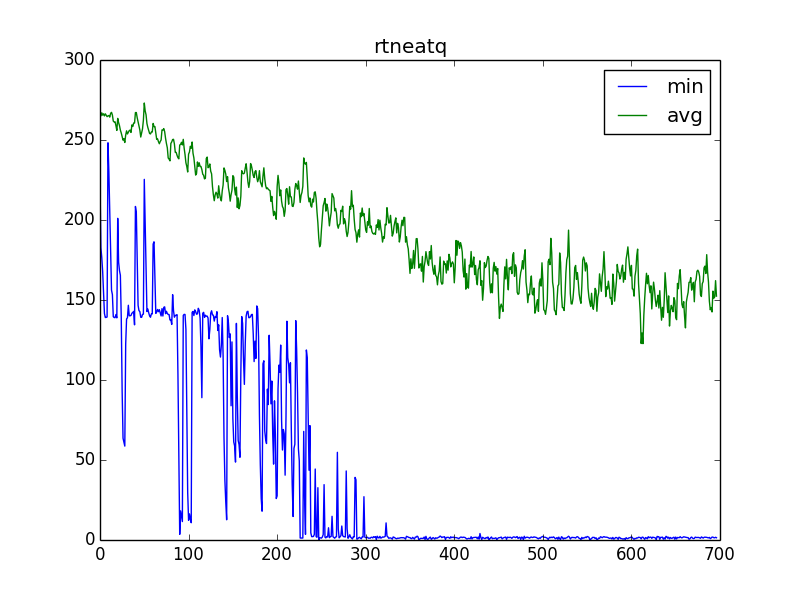
\includegraphics[width=\columnwidth]{wall_rtneatq.png}
  \caption{rtNEAT + Q Learning}
  \label{fig:wall_neatq}
\end{subfigure}
\caption{Approaching a flag with obstacles}
\label{fig:wall}
\end{figure*}

\section{Discussion and Future Work}
The results presented in Section~\ref{sec:exp} show that rtNEAT+Q converges more slowly than simple neuro-evolution in the simple task of approaching a flag without obstacles. Given the Lamarckian nature of the rtNEAT+Q algorithm, one might expect rtNEAT+Q to accelerate convergence by guiding agents closer to optimal policies during their lifetimes, though this does not appear to be the case. Consider that the learning phase of the rtNEAT+Q algorithm only produces error on the Q-value output for a single candidate action at a time. Essentially, networks are selected with some set of candidate action policies, and the learning phase learns which policy to use at any given step. There is little opportunity for learning to occur on the possible actions themselves, and would only occur in cases where NEAT evolves hidden units that feed forward to both Q-value outputs and action vector outputs. In this way, NEAT acts as a bottleneck, where networks must be evolved to have a useful action policy or set of action policies, and errors in the Q-value function cause deviations from optimal action policies, having the opposite of the desired effect on convergence.

Figures~\ref{fig:flag}-~\ref{fig:wall} show that Q learning does not perform well in our experiments. It is always a challenge for reinforcement learning in continuous domain. The implementation there is simply discretization the orientation to lots of intervals. It will cause a huge search space. Thus it is difficult to find the optimal solution by TD update. Also, on OpenNERO platform, the lifetime of each agent is related to the fitness to current environment. If the speed of learning is too low, they will be reset and consequently it is difficult for Q learning agents to get to the flag. 

Another problem with Q-learning that extends to rtNEAT+Q is the difficulty of exploration. Here, we use $\epsilon$-greedy selection. Each time the agents selects an action, it choose probabilistically between exploration and exploitation. With probability $\epsilon$, it will explore by selecting randomly from the available actions. With probability 1-$\epsilon$, it will exploit by selecting the greedy action. Such a mechanism may be effective in providing a balance between exploration and exploitation in domains in which each time step is significantly different from the last and actions cause major changes to future observations. However in continuous time domains such as OpenNERO, picking a random action some small percentage of the time will only cause minor fluctuations in behavior since it will usually be immediately followed by an optimal action. It's like exploration consists of walking just one step off the beaten path and then returning to it instead of taking another path entirely. 

When presented with the more complex task of navigating around an obstacle, rtNEAT+Q outperforms rtNEAT alone. The wall between the starting point of the agents and their target flag presents a local optima in their action policy, in which an agent might run directly towards the flag and become stuck against the wall. Stepping around the wall temporarily increases distance to the flag, but is required to reach the flag eventually and begin the processes of selecting agents that route around the obstacle, and learning new Q-values that reward routing around the wall. The learning phase used in rtNEAT+Q acts as sort of additional exploration mechanism, where noise or error in the Q-value function will cause repeated non-optimal action selection. By increasing the tendency to explore during agent lifetimes, agents are able to more effectively avoid local optima. Furthermore, it is possible that useful action policies may arise as compositions of simpler candidate actions from the selected networks. For instance a simple candidate may arise that just guides an agents directly towards the flag, but when the wall is hit, the Q-value selection mechanism begins to use another candidate that allows navigation around the obstacle. In this example each candidate represents a simple action policy that may be combined into a more effective overall policy. 

According to our results, rtNEAT+Q can successfully train neural network function approximators. However, rtNEAT+Q requires many more episodes to find good solutions than rtNEAT do in the same domain. Since each candidate network must be trained long enough to let Q-learning work, it has very high sample complexity. Moreover, for each episode, rtNEAT+Q also takes around 40\% more time than rtNEAT. The extra time is used to back propagate neural networks according to TD updates. However, such process is independent of the policy the agent is following, one network can be updated while another is controlling the agent. Furthermore, a network can be updated based on data saved from previous sample episodes, regardless of what policy was used during those episodes. Consequently,
it is not necessary to use different episodes to train each network. As shown in \cite{whiteson2006sample}, we could save data from the episodes used by the previous generation, each network in the population can be pre-trained off-line

Having implemented the relatively simple Lamarckian rtNEAT+Q algorithm, and examined its behavior, we may now consider future research in combining evolution and learning. A straightforward possibility would be to implement a Darwinian variant, in which the changes to the underlying networks caused by learning are not taken into account in the genomes being evolved by NEAT. Other work may include the development of new learning mechanisms that include exploration and learning in the action vector space instead of just Q-values, allowing for more effective learning. This would hopefully induce the desirable behavior of Lamarckian evolution accelerating convergence over simple evolution, even in simple domains, but may be more prone to local optima.

If agents are able to learn in a way that includes an effective exploration parameter, it may be very desirable to vary the exploration between agents in an evolved population and take advantage of that diversity in exploration. In short, it is likely to be very effective for there to be some agents that are highly exploratory, and others that are highly exploitative. Exploratory agents may discover new possibilities and route around even very difficult local optima. However as long as exploitative agents exist that will consistently achieve high fitness and be selected for future generations, there is little to no cost to concurrently having these exploratory agents while they search for new options, presumably at a cost to their own fitness.

The OpenNERO environment provides us with a great deal more than what has been used in this paper, including the ability to create much more complex optimization and learning tasks, including actual battle between multi-agent teams. This is a good opportunity to explore co-evolution, competitive evolution, or even multi-agent learning approaches such as social learning~\cite{tansey2012accelerating}.

\section{Conclusion}
Reinforcement learning is an appealing and empirically successful approach to finding effective
control policies in large probabilistic domains. There are three ways to solve the problem: evolution, TD update and their combination. Their performances depend on the properties of the task. According to our research and experiments, TD update is more suitable in discrete domains with limited states and actions. Evolution outperforms it in continuous domains and converges quickly in simple tasks. The combination of evolution and TD update can solve complex problems with better result than learning or evolution alone. It takes more time but it also evolves a function approximator during learning. In this project, rtNEAT+Q is implemented for combination of reinforcement learning in continuous domain and realtime evolution. It is tested in OpenNERO to train the agents to approach a flag. The experiments provide insight about the advantages of models related to task complexity.

\section*{Acknowledgements}
Thanks to Professor Risto Miikkulainen for his kind discussion with us about the project. Thanks to Kim Houck for her help with understanding OpenNERO platform.

\bibliographystyle{aaai}
\bibliography{report}



\end{document}
